Целью работы в текущем семестре было написание программного модуля для нахождения медиа-файлов (аудио, видео, изображение) и извлечения мета-данных.

\subsubsection{Введение}

На базе модуля, сканирующего изображения, была построена основа данного модуля. А именно --- проход по файлам с нужным расширением, считывание базовой информации о файле и вывод в XML формат.

Далее необходимо было изучить структуру мета-данных в медиа-файлах и возможность извлекать эти данные. В качестве начальных форматов тэгов были выбраны ID3v1, JFIF и RIFF. Эти типы мета-данных принадлежат к аудио, изображениям и видео соответственно.

Самым простым в реализации оказался тип ID3v1, с которого и было начато исследование.

\subsubsection{ID3v1}

ID3v1 --- формат метаданных, наиболее часто используемый в звуковых файлах в формате MP3. Он содержит данные о названии трека, альбома, имени исполнителя и годе выпуска. Сами эти данные располагаются в конце файла MP3 и имеют структуру, представленную в таблице~\ref{tab:id3v1}).

Блок-схема алгоритма считывания ID3v1 представлена на рисунке~\ref{bokov_1:bokov_1}. Как следствие, в XML-файле теперь эти данные имеют следующее представление (рис.~\ref{bokov_2:bokov_2}).

\begin{table}[ht]
\caption{Структура ID3v1}
\label{tab:id3v1}
\begin{center}
\begin{tabularx}{\linewidth}{|l|X|}
\hline
Поле & Размер (в байтах) \\
\hline
Заголовок & 3 (всегда равен <<TAG>>) \\
\hline
Название трека & 30 \\
\hline
Имя исполнителя & 30 \\
\hline
Название альбома & 30 \\
\hline
Год выпуска & 4 \\
\hline
Комментарии & 30 \\
\hline
Жанр & 1 \\
\hline
\end{tabularx}
\end{center}
\end{table}

\begin{figure}[h!]
\center{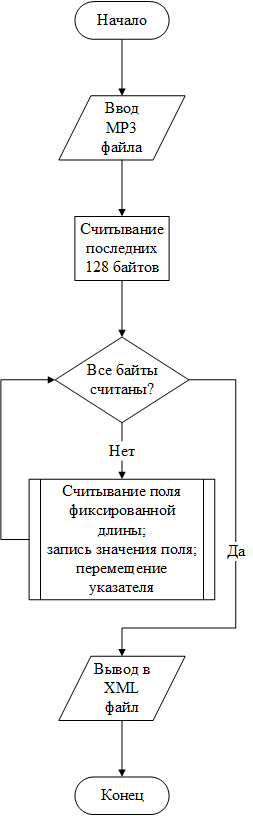
\includegraphics[width=0.3\linewidth]{bokov_1}}
\caption{Блок-схема алгоритма считывания ID3v1}
\label{bokov_1:bokov_1}
\end{figure} 

\begin{figure}[h!]
\center{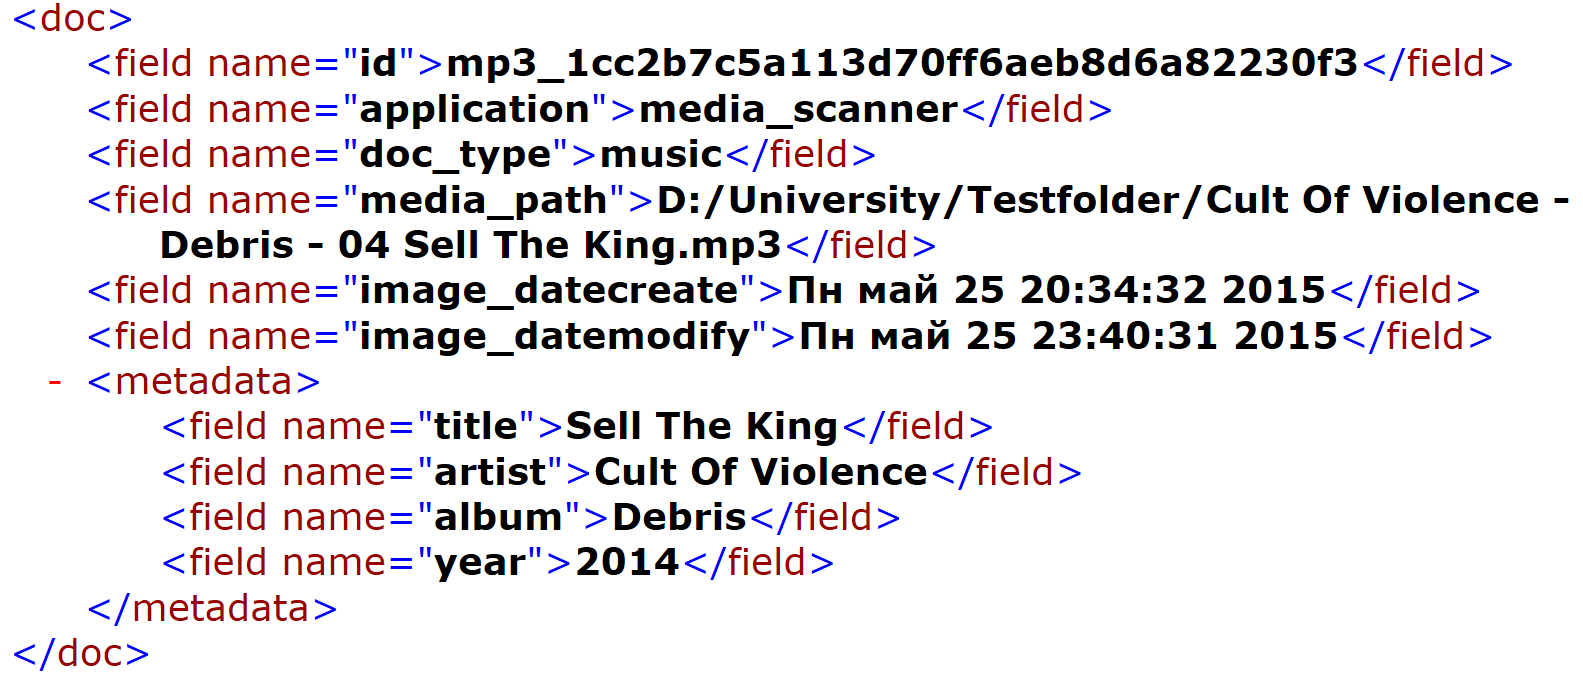
\includegraphics[width=0.6\linewidth]{bokov_2}}
\caption{Результат вывода в XML-файл}
\label{bokov_2:bokov_2}
\end{figure}

\clearpage

\subsubsection{JFIF}

JPEG File Interchange Format (JFIF) --- формат файлов-изображений. Является несколько менее совершенной версией формата EXIF, однако так же позволяет хранить данные об изображении, такие как разрешение изображения, плотность пикселей и данные о миниатюре изображения. Формат представлен в следующем виде ( ~\ref{tab:jfif}).


Блок-схема алгоритма считывания JFIF представлена на рисунке~\ref{bokov_3:bokov_3}, полученный результат в XML-формате --- на рисунке~\ref{bokov_4:bokov_4}.

\begin{table}[ht]
\caption{Структура JFIF}
\label{tab:jfif}
\begin{center}
\begin{tabularx}{\linewidth}{|l|X|}
\hline
Поле & Размер (в байтах) \\
\hline
Маркер APP0 & 2 \\
\hline
Длина & 2 \\
\hline
Идентификатор & 5 \\
\hline
Версия & 2 \\
\hline
Единица измерения плотности & 1 \\
\hline
Плотность по X & 2 \\
\hline
Плотность по Y & 2 \\
\hline
Ширина миниатюры (tw) & 1 \\
\hline
Высота миниатюры (th) & 1 \\
\hline
Данные миниатюры & 3 * tw * th \\
\hline
\end{tabularx}
\end{center}
\end{table}

\begin{figure}[h!]
\center{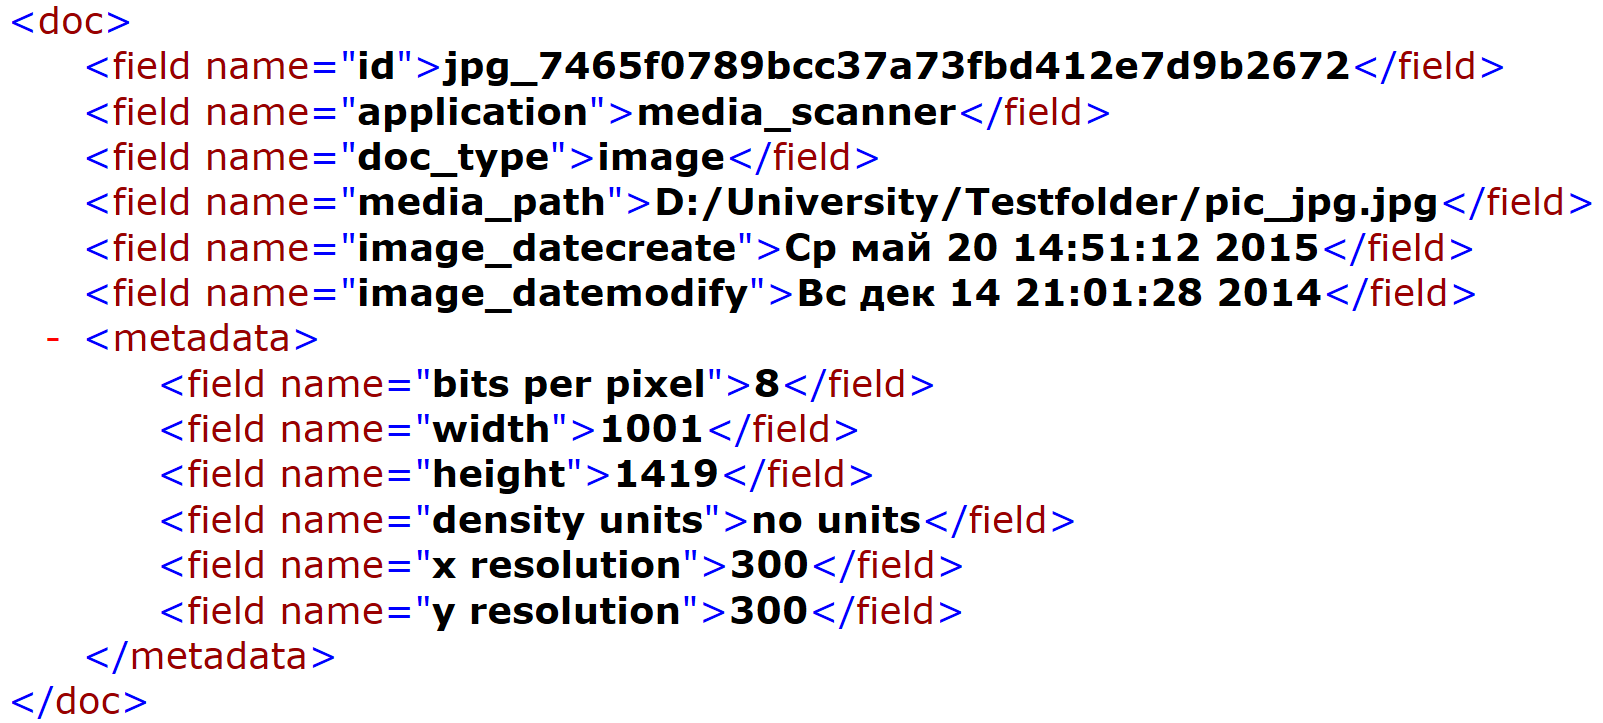
\includegraphics[width=0.7\linewidth]{bokov_4}}
\caption{JPG в XML}
\label{bokov_4:bokov_4}
\end{figure}

\begin{figure}[h!]
\center{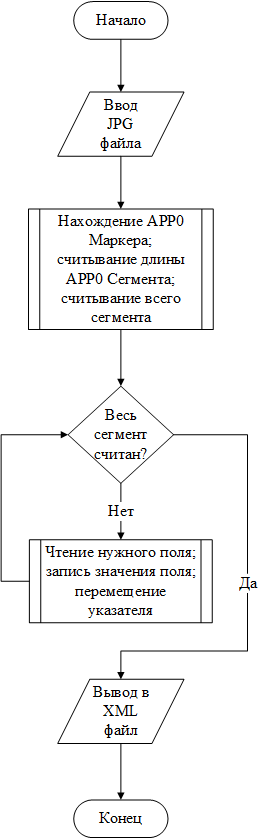
\includegraphics[width=0.4\linewidth]{bokov_3}}
\caption{Считывание JFIF}
\label{bokov_3:bokov_3}
\end{figure} 

\clearpage

\subsubsection{RIFF}

Resource Interchange File Format (RIFF) --- один из форматов файлов-контейнеров для хранения потоковых мультимедиа-данных. Наиболее известными форматами, использующими RIFF в качестве контейнера, является AVI.
Основной концепцией формата является chunk -- порция данных с заголовком и сигнатурой, указывающей на содержимое chunk`а.
В chunk`е strh хранятся общие данные о потоке и определение того, какого типа этот поток (аудио, видео, текст или midi). Соответственно, в его дочернем chunk`е (strf) содержится следующая информация, если это видео (таблица~\ref{tab:strf}).

\begin{table}[ht]
\caption{Структура strf (vids)}
\label{tab:strf}
\begin{center}
\begin{tabularx}{\linewidth}{|l|X|}
\hline
Номер байта & Метаданные \\
\hline
0-3 & STRF \\
\hline
4-7 & Размер \\
\hline
8-11 & Ширина \\
\hline
12-15 & Высота \\
\hline
16-19 & Bit planes \\
\hline
20-23 & Кол-во бит на пиксель \\
\hline
24-27 & Сжатие бит \\
\hline
28-31 & Размер изображения \\
\hline
32-35 & Горизонтальное разрешение \\
\hline
36-39 & Вертикальное разрешение \\
\hline
40-43 & Показатель цвета \\
\hline
44-49 & Количество важных цветов \\
\hline
\end{tabularx}
\end{center}
\end{table}

Если же это аудио, то информация будет выглядеть следующим образом (таблица~\ref{tab:auds}).

\begin{table}[ht]
\caption{Структура strf(auds)}
\label{tab:auds}
\begin{center}
\begin{tabularx}{\linewidth}{|l|X|}
\hline
Номер байта & Метаданные \\
\hline
0-3 & STRF \\
\hline
4-7 & Размер \\
\hline
8-9 & Компрессор \\
\hline
10-11 & Каналы \\
\hline
12-13 & Частота дискретизации \\
\hline
14-15 & Байты в секунду \\
\hline
16-17 & Block align \\
\hline
18-19 & Бит на семпл \\
\hline
\end{tabularx}
\end{center}
\end{table}

Алгоритм обработки RIFF --- рисунок~\ref{bokov_5:bokov_5}, вывод в XML-файл --- рисунок~\ref{bokov_6:bokov_6}. 

\begin{figure}[h!]
\center{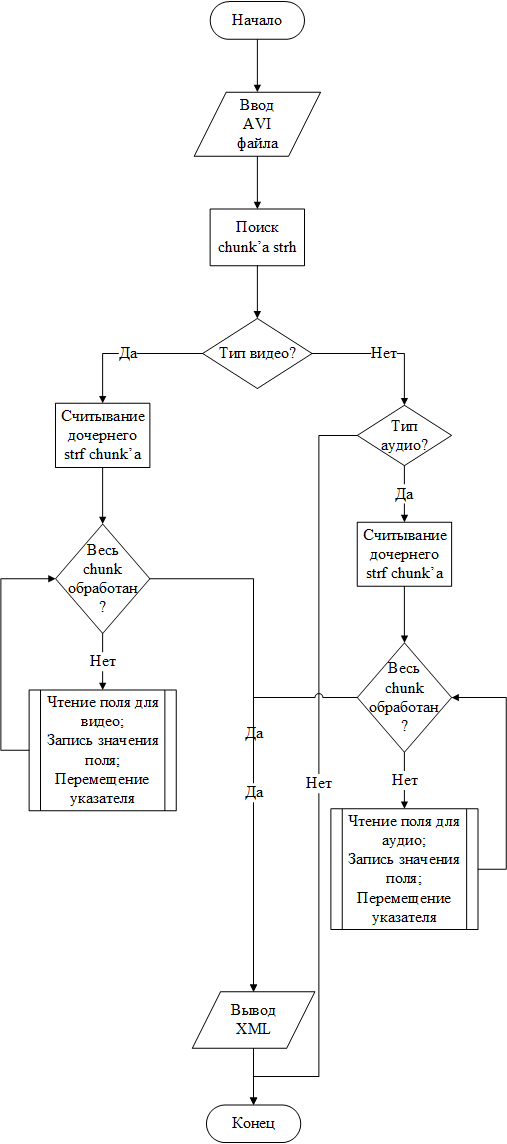
\includegraphics[width=0.5\linewidth]{bokov_5}}
\caption{Алгоритм обработки RIFF}
\label{bokov_5:bokov_5}
\end{figure} 

\begin{figure}[h!]
\center{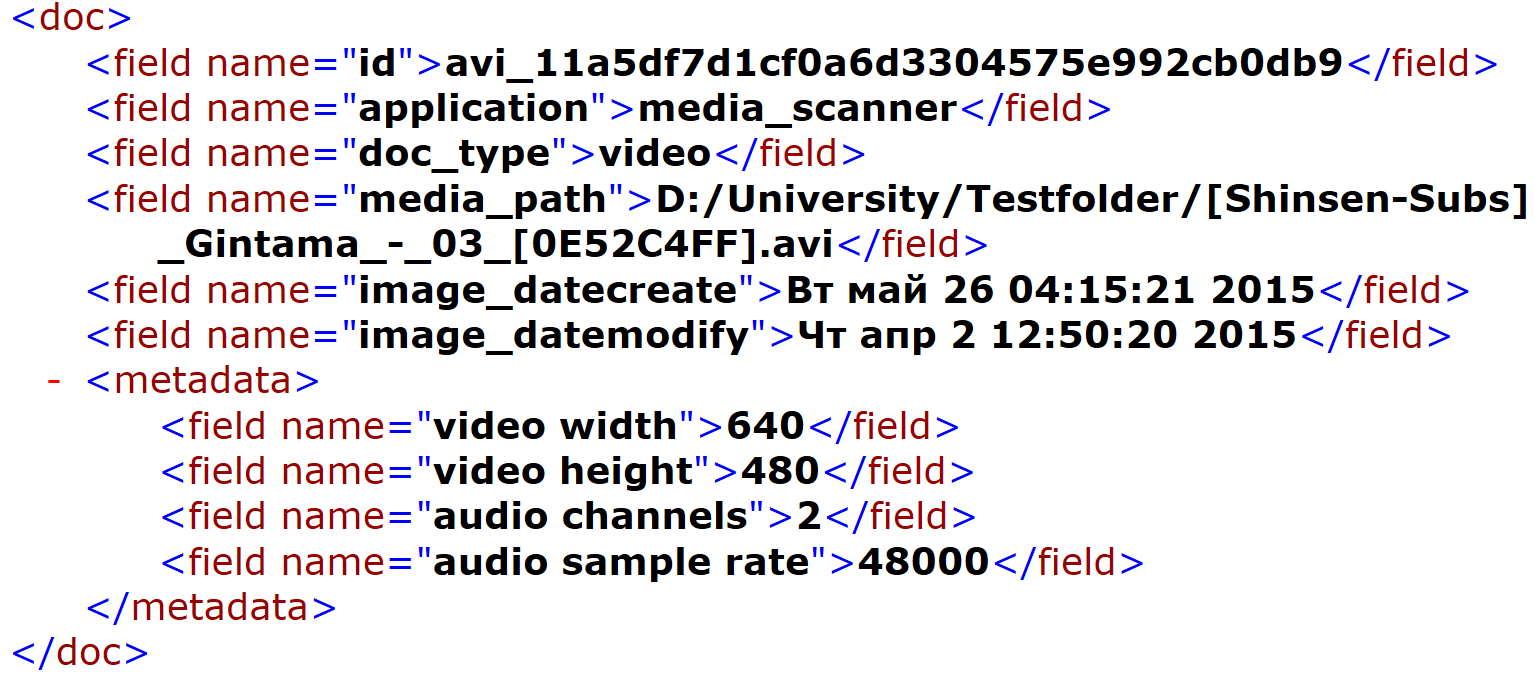
\includegraphics[width=0.4\linewidth]{bokov_6}}
\caption{Результат в XML}
\label{bokov_6:bokov_6}
\end{figure}

\subsubsection{Задачи на следующий семестр}

На данный момент программа является модульной, что позволяет без особого труда добавлять в нее поддержку новых расширений и типов форматов мета-данных. В будущем планируется добавление таких форматов мета-данных, как mkv, exif, id3v2, и поддержка еще большего количества расширений, а также усовершенствование работы программы с уже имеющимися форматами.

В этом семестре реализовано:

\begin{itemize}
  \item рекурсивный обход директорий;
  \item чтение формата мета-данных для видео RIFF;
  \item чтение полей тегов формата JFIF;
  \item чтение информации об mp3 из контейнера ID3v1.
\end{itemize}

\clearpage
